\documentclass[../main.tex]{subfiles}
\begin{document}


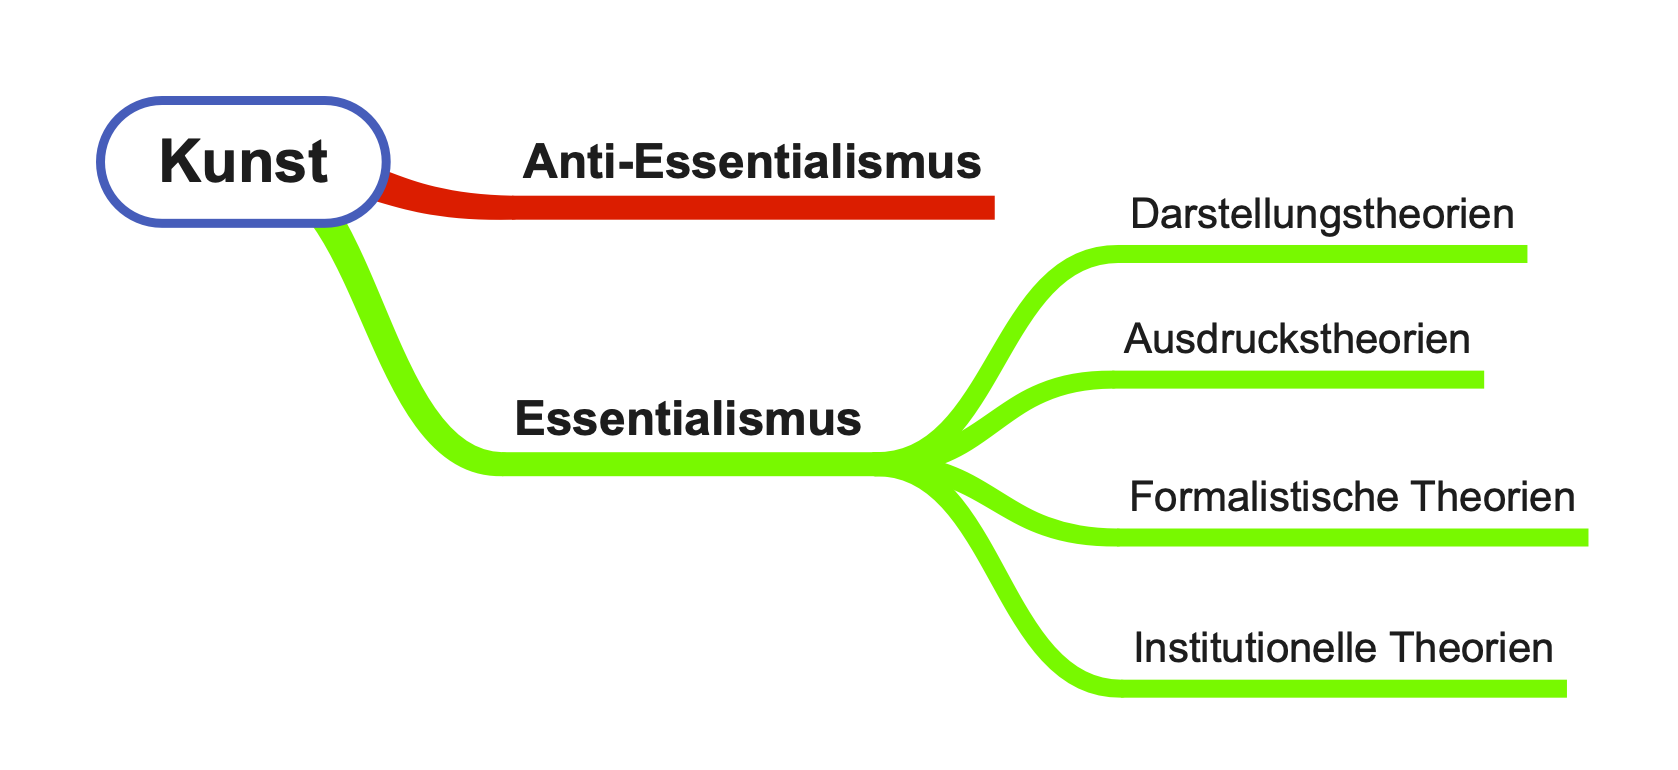
\includegraphics[width=\textwidth]{images/Kunst_Uebersicht.png}

\section{Definition von Kunst}
Die Philosophische Disziplin, die die Kunst als Gegenstand hat, ist die Ästhetik. Diese beschäftigt sich mit dem Schönen. Dabei ist das schöne nacht klassischer Auffassung, das, was ästhetisch ist und das sind Kunstwerke. Aber was sind Kunstwerke, resp. welche notwendigen Bedingungen müssen diese Erfüllen, damit diese hinreichend für ein Kunstwerk sind?

Bei der Kunstklassifizierung spielen unterschiedliche geschichtliche Epochen eine grosse Rolle. So sind je nach Epoche gewisse Dinge als Kunstwerk klassifiziert und andere nicht (die es teilweise noch nicht einmal gibt). 

\section{Darstellungstheorien von Kunst}
Die Begrifflichkeit <<Kunst>> wurde im 18. Jahrhundert geprägt. Plan und Aristoteles hatten keine solche! Es wurde klassifiziert in die fünf schönen Künste Architektur, Bildhauerei, Malerei, Musik und Poesie. 

\paragraph{These} Etwas ist ein Kunstwerk gdw. es etwas darstellt/repräsentiert.
\paragraph{Probleme} 
\begin{enumerate}
	\item Was genau ist darstellen? Wenn es etwas ähnlich sieht? Dann würden Romane ja nicht zählen!
	\item Ähnlichkeit ist unzureichend, selbst für bildliche Kunst. So ist z.B: ein abstraktes Bild kaum ähnlich zu irgendwas. Ähnlichkeit ist also nicht notwendig (muss keine Ähnlichkeit haben) und nicht hinreichend.
	\item Wie kann eine Ähnlichkeitsbeziehung zwischen Kunstwerken und einem fiktiven Gegenstand bestehen?
	\item Es scheint so, als wäre Darstellung keine notwendige Bedingung für Kunst
	\item Darstellung ist nicht hinreichend für Kunst (technische Zeichnungen, Urlaubsfotos, Sachbücher)
\end{enumerate}

\subsection{Konventionalismus}
\paragraph{These} Etwas stellt etwas anderes dar gdw. es eine Konvention gibt, die besagt, dass dieses etwas dieses andere etwas darstellt. 
\paragraph{Argumente}
\begin{enumerate}
	\item Es ist plausibel, dass literarische Werke in diesem Sinne darstellend sind (aufgrund Konventionen können Zeichen bestimmte Sachverhalte repräsentieren)
\end{enumerate}
\paragraph{Probleme}
\begin{enumerate}
	\item Wenn Darstellungsbeziehungen auf einer Konvention beruhen, wie kommt es, dass wir diese beherrschen? Wer hat also die Konvention erfunden, eine Form einem realen Gegenstand entspricht/auf diesen verweist? Denn offensichtlich beherrschten bereits Höhlenbewohner diese darstellenden Konventionen und diese haben sie offensichtlich nicht kulturell gelernt.
	\item Es scheint so, als wäre Darstellung keine notwendige Bedingung für Kunst
	\item Darstellung ist nicht hinreichend für Kunst (technische Zeichnungen, Urlaubsfotos, Sachbücher)
\end{enumerate}

\section{Ausdruckstheorien von Kunst}
\paragraph{These} Etwas ist ein Kunstwerk gdw. es eine Emotion ausdrückt.
\paragraph{Probleme} 
\begin{enumerate}
	\item Was bedeutet es, dass etwas Gefühle ausdrückt? Wenn die herstellende Person bei der Herstellung Gefühle hatte? Oder wenn diese Gefühle in der herstellenden Person massgeblich die Gestaltung des Werkes beeinflusst hat?
	    
	    Aber das ist selbst bei expressiven Künstler:innen nicht immer der Fall!
	\item Was bedeutet es, dass etwas Gefühle ausdrückt? Wenn es in den Betrachtern (tendenziell) Gefühle einer Art hervorruft?
	    
	    Aber was ist, wenn es bei einigen ganz andere Gefühle auslöst?
	\item Es ist nicht notwendig, dass alle Kunstwerke Gefühle ausdrücken müssen.
	\item Eine Gefühlsäusserung ist nicht hinreichend dafür, ein Kunstwerk zu sein.
\end{enumerate}

\section{Formalistische Theorien von Kunst}
\paragraph{These} Etwas ist ein Kunstwerk gdw. es bestimmte formale Qualitäten hat
\paragraph{Erklärung} Gemäss Clive Bell (1881-1964) haben alle (visuellen) Kunstwerke folgende signifikanten formalen Qualitäten:
\begin{enumerate}
	\item es hat eine signifikante Form bestehen aus Linien, Flächen, etc. deren Kombination eine besondere Art von Emotionen, die ästhetischer Natur, auslösen. Dabei wird aber vorausgesetzt, dass es solch eine Emotion gibt und die Ursache dieser Emotion ein formales Merkmal von allen visuellen Kunstwerken ist.
\end{enumerate}
\paragraph{Problem}
\begin{enumerate}
	\item Gibt es besondere ästhetische Emotionen wirklich?
	\item Lässt sich die Form, die diese Emotion verursacht, irgendwie spezifizieren?
	\item Sind schlechte Kunstwerke keine Kusntwerke?
\end{enumerate}

\section{Institutionelle Theorien von Kunst}
\paragraph{These} Etwas ist ein Kunstwerk gdw. die Kunstwelt dieses als Kunstwerk anerkannt/behandelt.
\paragraph{Erklärung} Diese Theorie besagt, dass Kunstwerke nicht etwas spezielles an sich haben, sondern aufgrund extrinsischer Merkmale als Kunstwerke eingestuft werden (Relation zur Kunstwelt, darunter alle Institutionen, die etwas mit Kunst zu tun haben).

Der einflussreichste Vertreter dieser Theorie, George Dickie (ein anderer wäre Arthur Danto), stellt klar, dass etwas ein Kunstwerk ist, wenn eine oder mehrere Personen im Namen der Kunstwelt dem Werk den Status eines Wertobjektes verliehen haben.  
\paragraph{Probleme}
\begin{enumerate}
	\item Muss wirklich jedes Kunstobjekt den Status des Werobjektes haben?
	\item Und welche Personen zählen zur Kunstwelt?
	\item Kann Kunst nicht auch ausserhalb der Institutionen der Kunstwelt geschaffen werden?
\end{enumerate}

\section{Anti-Essentialismus}  
\paragraph{Erklärung} Der Anti-Essentialismus (Vertreter: Morris Weitz, Paul Ziff) folgt Wittgensteins Philosophie der Sprache und definiert Kunstwerke aufgrund von Familienähnlichkeiten als Kunst. Das heisst, ein Kunstwerk ist ein solches, wenn es bestimmte Gemeinsamkeiten mit anderen Werken hat, die wiederum gewisse Gemeinsamkeiten mit wiederum anderen Werken hat etc. Somit widerspricht der Anti-Essentialismus dem kunstästhetischen Essentialismus, der besagt, dass es ein Wesen der Kunst (universelles Merkmal) gibt, welches Kunst von nicht-Kunst unterscheidet.
\paragraph{Argumente}
\begin{enumerate}
	\item Nur weil wir verschiedene Dinge in einer Kategorie zuordnen (z.B. Kunst), heisst das nicht, dass diese Dinge auch effektiv Gemeinsamkeiten haben
	\item Morris Weitz: Es gibt nicht, dass alle die Gegenstände, die wir als Kunstgegenstände anerkennen, gemeinsam haben. Und gäbe es etwas solches, so wäre es in der Natur der Kunst, dieses zu umgehen (Kunst entwickelt sich weiter).
\end{enumerate}

\end{document}